\section{Study area and data sources}\label{sec:study_area}

% \subsection{Areas of interest}

\paragraph{Mississippi, USA}
The overarching goal of this work is to develop a 1 m resolution land cover map for the state of Mississippi to facilitate high-fidelity land analysis.
Mississippi is located in the southeastern United States, and is home to a wide range of land cover types.
The region's humid subtropical climate and fertile soils in the Mississippi River Delta support a variety of agricultural activities~\cite{mississippistateuniversityextensionMississippiLandResource}, while the remainder of the state is characterized by forests and woodlands which comprise the majority of land cover in the state~\cite{unitedstatesgeologicalsurveyAnnualNationalLand}.
The Gulf coast region is home to a sprawling urban network intertwined with herbaceous wetlands and barren beaches~\cite{englishLandCoverChange2011}.
The state's diverse land cover types, geographical position along the Mississippi River and Gulf Coast, and economic dependence on agriculture and natural resources make the need for accurate land cover information at high spatial resolution a priority to support natural resource management, agricultural planning, and environmental monitoring efforts.

\paragraph{Virginia, USA}
% In order to validate our proposed stratification approach, we also invesrtigate the performance of the proposed method using an existing land cover dataset.
A secondary objective of this work is to introduce and validate a novel approach to stratification for selecting patch-based training samples for semantic segmentation of land cover.
For this purpose, we use the portion of the Chesapeake Bay watershed (CBW) located in Virginia as a case study to validate our proposed stratification approach.
The CBW is a \SI{168,000}{\kilo \meter \squared} drainage basin along the Eastern Seaboard of the United States, stretching from central VA at its southernmost point to central NY at its northernmost.
Like Mississippi, the CBW is comprised of a large amount of forests and wetlands, while having some agricultural areas.
Notably, the region has been the focus of rapid urbanization in recent decades, particularly along the Eastern Shore, where land cover conversion from agricultural, wetlands, and forested areas to urban areas has been a significant concern for environmental management and conservation efforts.
The region's large population, economic importance, and ecological significance have led to the CBW being a central focus of numerous land use and land cover mapping efforts for environmental monitoring purposes~\cite{jantzUrbanizationLossResource2005, bhattWaterQualityImpacts2023, cooperChesapeakeBayWatershed1995}.
% The Chesapeake Bay Program (CBP) land cover dataset is used to provide ground truth data for this phase of the study.
% The CBP land use and land cover products are among the largest meter-scale land cover datasets in the United States, and are produced by the Chesapeake Conservancy as part of a cooparative agreement between the US Geological Survey and the US Environmental Protection Agency~\cite{claggettChesapeakeBayLand2025}.
% The 2024 edition provides a 56-class land use product at \SI{1}{\meter} resolution over the Chesapeake Bay watershed, which includes portions of six states (Delaware, Maryland, New York, Pennsylvania, Virginia, and West Virginia) and the District of Columbia for the years 2013/2014, 2017/2018, and 2021/2022.


\subsection{Imagery and land cover dataset}\label{sec:data}

\paragraph{National Agriculture Imagery Program (NAIP)}\label{sec:data:naip}
The primary remote sensing data used in this work is aerial imagery sourced from the USDA's National Agriculture Imagery Program (NAIP)~\citep{earthresourcesobservationandscienceeroscenterNationalAgricultureImagery2017}.
NAIP provides a publicly available archive of high-resolution multispectral imagery over CONUS, with a spatial resolution of \SIrange{0.3}{1}{\meter} and a four-band spectral resolution (near-infrared, red, green, and blue).
NAIP imagery is collected on a state-by-state basis during the agricultural growing season, and each state is imaged once every 2--3 years.
We use 2023 NAIP imagery over Mississippi, and 2021 NAIP imagery over the CBW region in Virginia.
Color-infared (CIR) composites are generated using the near-infrared, red, and green bands for both study areas to emphasize vegetation features in the imagery -- the blue band is excluded from analysis.
Additionally, we downsample imagery to \SI{1}{\meter} resolution to match the resolution of the desired final land cover product.


\paragraph{National Land Cover Database (NLCD)}\label{sec:data:nlcd}

The stratification approach proposed in this work relies on an existing land cover product to select strata from which training samples are drawn.
For this purpose, we opt for the USGS's National Land Cover Database (NLCD) to provide the necessary land cover information for stratification. 
The NLCD has historically been among the most widely used land cover datasets in the United States, and has seen a plethora of applications in human and ecosystem health studies, urban planning, natural hazard assessment, hydrology, and land management studies~\citep{sohlThirtyYearsUS2025}.
The latest version of the NLCD (Annual NLCD) provides a yearly 20 class land cover product primarily derived from Landsat imagery at \SI{30}{\meter} resolution from 1985 to 2024~\citep{unitedstatesgeologicalsurveyAnnualNationalLand2025}.
While the spatial resolution of the NLCD land cover product is substantially coarser than the \SI{1}{\meter} land cover product we aim to produce, the NLCD provides an accurate and comprehensive land cover product at a national scale and has a history of consistent use in the literature, making it a suitable choice to provide land cover information to help guide the stratification process.
To align with the collection year of the NAIP imagery used in this work, we use 2023 data for Mississippi, and 2021 data for the CBW region.

\paragraph{CBW Land Use/Land Cover (CBLC)}\label{sec:data:cblc}

In order to validate our proposed stratification approach, a source of ground truth VHSR land cover data is required to assess the performance of models trained using our proposed method and compare them to models trained using other sampling strategies.
For this purpose, we utilize the Chesapeake Bay Land Use/Land Cover (CBLC) dataset, which provides a \SI{1}{\meter} resolution 56-class land use product over the CBW region.
The CBLC dataset is among the most extensive and detailed VHSR land cover datasets in the United States available to the public, and is produced by the Chesapeake Conservancy as part of a cooperative agreement between the US Geological Survey and the US Environmental Protection Agency~\citep{claggettChesapeakeBayLand2025}.
The land cover product is primarily derived form NAIP imagery and high-resolution LiDAR-derived elevation data along with a myriad of ancillary geospatial datasets using a combination of machine learning and rule-based classification techniques~\citep{mcdonaldChesapeakeBayLand2025}.
As the land cover product relies on NAIP imagery, the actual years of coverage vary across the CBW depending on the year in which each state was imaged by NAIP: the 2024 edition of the CBLC dataset provides data for the years 2013/2014, 2017/2018, and 2021/2022~\citep{claggettChesapeakeBayLand2025}.
We use the 2021/2022 edition of the CBLC dataset, as we are only concerned with the portion of the CBW located in Virginia, which was imaged in 2021.
A visualization of the two areas of interest and the data sources used in this work is provided in Figure~\ref{fig:study_areas}.

\begin{figure}[H]
    \centering
    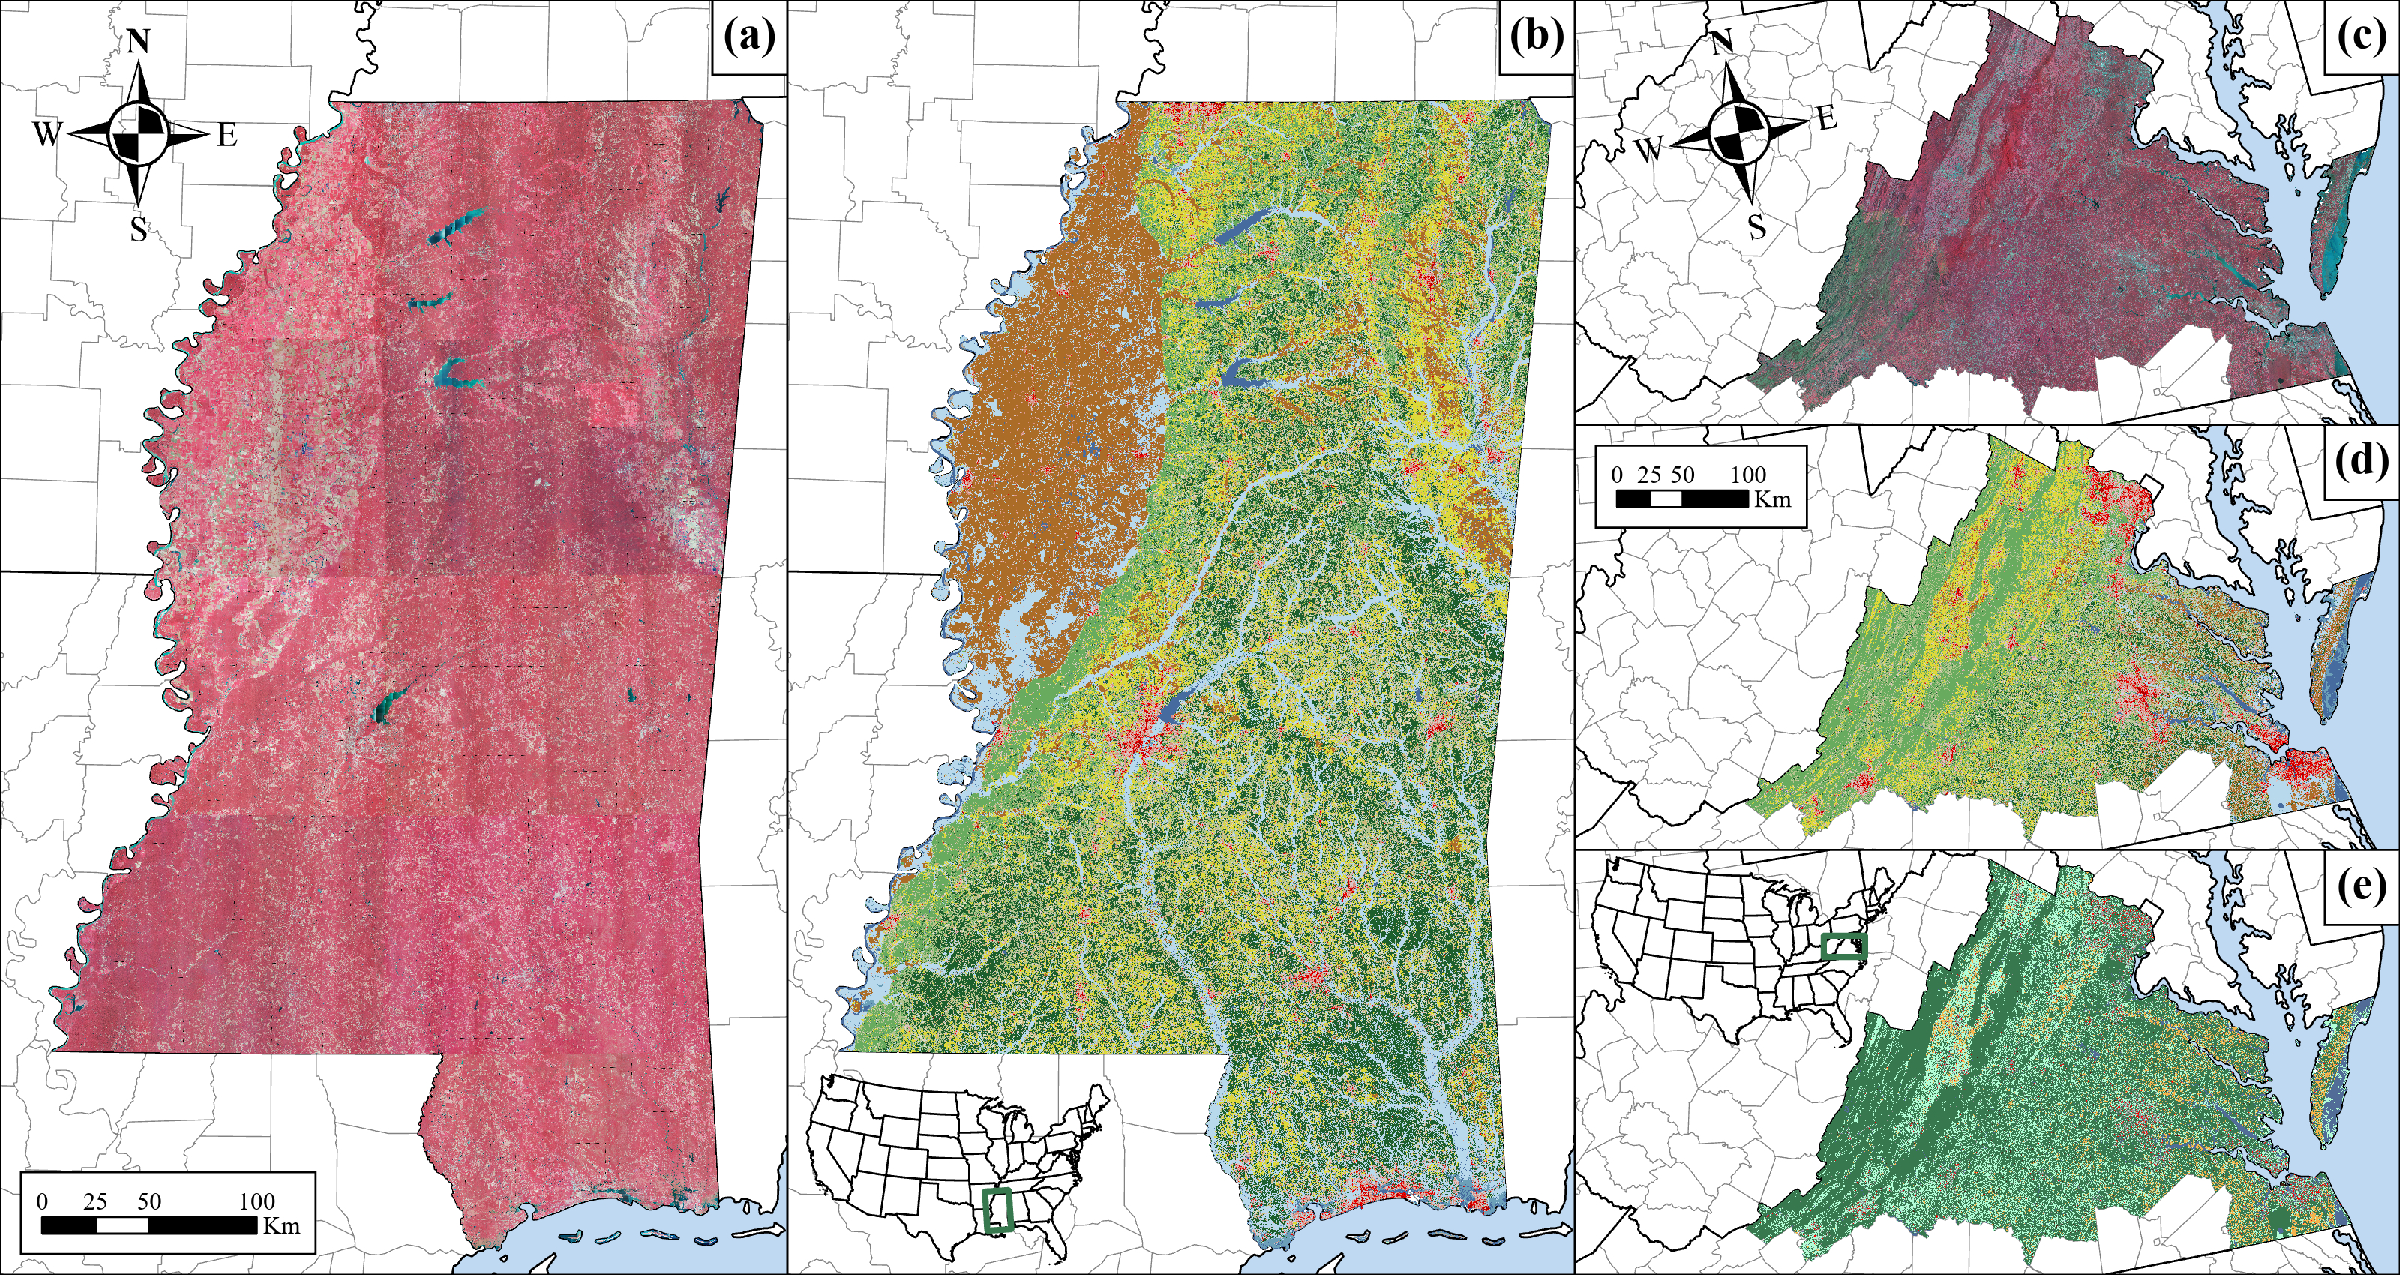
\includegraphics[width=\textwidth]{images/Study_Area.pdf}
    % \caption{Study areas and data sources used in this work: (a) NAIP imagery over the primary study area in Mississippi (b) NLCD 2021 land cover for Mississippi, USA; (c) NAIP imagery over the Chesapeake Bay watershed in Virginia, USA. Imagery over this area will be used to validate a sampling strategy given \SI{1}{\meter} land cover data is pubclicly available for this region; (d) NLCD 2022 land cover map over the Chesapeake Bay watershed in Virginia, USA; (e) CBLC \SI{1}{\meter} land cover map over the Chesapeake Bay watershed in Virginia, USA.}\label{fig:study_areas}
    \caption{The two study areas and corresponding data sources used in this work. (a, b) NAIP imagery and NLCD 2021 land cover for the primary area of interest in Mississippi, USA. (c, d, e) NAIP imagery, NLCD 2022, and \SI{1}{\meter} CBLC data for a subset of the Chesapeake Bay watershed located in Virginia, USA. \note{MOVE VA MAPS SO FULL AOI IS IN FRAME}}\label{fig:study_areas}
    
\end{figure}